\section{The PID control law}
\subsection{}

\begin{frame}
\frametitleTC{The overall law}
\framesubtitleTC{recap in preparation for the implementation}
\myPause
 \begin{itemize}[<+-| alert@+>]
 \item The control signal $u(k)$ is the sum of the Proportional (P), the Integral (I)\\
       and the derivative (D) action:
       \begin{displaymath}
        u(k) = u_P(k)+u_I(k)+u_D(k).
       \end{displaymath}
 \item Some action may not be present, giving rise to the P, I, PI, PD laws -- with\\
       obvious meaning -- besides the complete PID one (D and ID make little\\
       -- if any -- sense in practice, we omit further discussions).
 \item We shall now study the three actions, then deal with actuator limits,\\
       and finally move to the algorithm.
 \end{itemize}
\end{frame}

\begin{frame}
\frametitleTC{The P action}
\framesubtitleTC{}
\myPause
 \begin{itemize}[<+-| alert@+>]
 \item The P action $u_P(k)$ is computed as
       \begin{displaymath}
        u_P(k) = K e(k).
       \end{displaymath}
 \item Its role is to respond \TC{promptly} to an error variation.
 \item Since there is no dynamics, that response is in fact instantaneous\\
       (if not for computation delay and machine-related timing facts\\
       at large).
 \end{itemize}
\end{frame}

\begin{frame}
\frametitleTC{The I action}
\framesubtitleTC{}
\myPause
 \begin{itemize}[<+-| alert@+>]
 \item The I action $u_I(k)$ is computed as
       \begin{displaymath}
        u_I(k) = u_I(k-1) + \frac{KT_s}{T_i} e(k).
       \end{displaymath}
 \item Its role is to guarantee \TC{zero steady-state error}.
 \item At steady state everything (including $u_I$) is constant, and therefore\\
       the error must be zero because in the opposite case $u_I$ would vary.
 \item In general, if your control scheme has to ensure that some variable\\
       is zero at steady state, just make that variable the input of an\\
       integrator. 
 \end{itemize}
\end{frame}

\begin{frame}
\frametitleTC{The D action}
\framesubtitleTC{}
\myPause
 \begin{itemize}[<+-| alert@+>]
 \item The D action \TC{in the CT domain} is expressed as
       \begin{displaymath}
        u_D(t) = K T_d \frac{de(t)}{dt}
       \end{displaymath}
       where $T_d$ is called the \TC{derivative time}.
 \item Its role is to attempt to \TC{anticipate the error} over a horizon $T_d$ in the future.
 \item Interpretation (and \emph{caveat} to not make $T_d$ too large):
       \begin{center}
        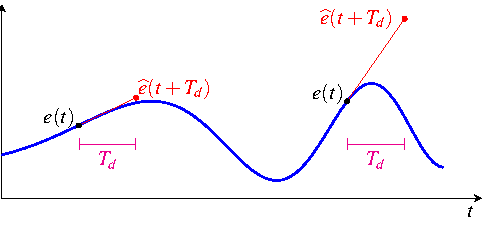
\includegraphics[width=0.45\columnwidth]{./Unit-06/img/D-action-interpretation.pdf}
       \end{center}
 \end{itemize}
\end{frame}

\begin{frame}
\frametitleTC{The D action}
\framesubtitleTC{}
\myPause
 \begin{itemize}[<+-| alert@+>]
 \item Sometimes the D action may respond too nervously, and therefore it is in fact computed as
       \begin{displaymath}
        u_D(k) = \beta u_D(k-1) + (1-\beta) K T_d \frac{e(k)-e(k-1)}{Ts}, \quad 0 < \beta < 1.
       \end{displaymath}
 \item In this course we provide no notion of \TC{frequency response} -- another hook for the\\
       interested -- but it should be intuitive that if $u_D(k)$ contains a fraction\\
       $\beta$ of $u_D(k-1)$ while the new input's contribution only weighs $1-\beta$,\\
       this combination acts as a \TC{lowpass filter}, i.e., smooths out the abrupt\\
       variations of $u_D$ that the input would otherwise provoke.
 \item In $z$ form we thus have
       \begin{displaymath}
        \frac{u_D(k)}{e(k)} = \frac{1-\beta}{z-\beta} \frac{K T_d}{T_s} \frac{z-1}{z}.
       \end{displaymath}
 \end{itemize}
\end{frame}

\begin{frame}
\frametitleTC{The D action}
\framesubtitleTC{}
\myPause
 \begin{itemize}[<+-| alert@+>]
 \item For reasons we do not have the time to fully discuss here (but ask if interested)\\
       it is convenient to set
       \begin{displaymath}
        \beta = \frac{T_d}{T_d+NT_s}, \qquad N>0,
       \end{displaymath}
       in a nutshell because doing so
       \begin{itemize}[<+-| alert@+>]
       \item the pole $\beta$ of the $u_D/e$ transfer function is surely in the range $(0,1)$,
       \item if $T_d=0$ (PI only) $\beta$ vanishes as well,
       \item parameter $N$ is a good knob to control the amount of smoothing applied\\
             to $u_D$ (higher $N$ means lower $\beta$, thus less of $u_D(k-1)$ in $u_D(k)$, thus\\
             less smoothing --- and clearly \textit{vice versa}). 
       \end{itemize}
 \item We are now ready for a PID ``quasi-algorithm''.
 \item In fact now we write just the essentials and then, after discussing\\
       control limits, we get to the real thing, also introducing some\\
       practically useful additions.
 \end{itemize}
\end{frame}

\begin{frame}[fragile,label={pag:PID-quasi-alg}]
\frametitleTC{A PID quasi-algorithm}
\framesubtitleTC{to be executed periodically with timestep $T_s$}
\myPause
 \begin{verbatim}
  e      = w-y;
  up     = K*e;
  ui     = ui_old+K*Ts/Ti*e;
  ud     = beta*ud_old+(1-beta)*K*Td/Ts*(e-e_old);
  u      = up+ui+ud;
  e_old  = e;
  ui_old = ui;
  ud_old = ud;
 \end{verbatim}
\end{frame}

